\chapter{Khối lượng fermion: chirality, các tương tác Yukawa và neutrino Majorana}

\lectureoverview{Trước hết ta dựng lại cơ chế Higgs của boson chuẩn trong một lý thuyết mô hình đồ chơi \(U(1)\), rồi đặt câu hỏi song song đối với fermion. Khối lượng Dirac trộn các trường chiral trái và phải, nhưng tương tác yếu gán cho chúng các điện tích khác nhau và vì thế cấm một khối lượng trần. Một tương tác Yukawa với trường Higgs tôn trọng đối xứng; sau khi trường Higgs nhận một giá trị chân không, chính tương tác đó trở thành khối lượng fermion và một liên kết Higgs--fermion đo được. Phần cuối đi theo logic này sang khối lượng neutrino, các hạt nặng khả dĩ không được bảo vệ, động học tia vũ trụ, quán tính tương đối tính và hấp dẫn.}

Mục đích của phần ôn mở đầu không chỉ đơn thuần là lặp lại bài giảng trước. Ta cần một ý từ đó ở dạng có thể chuyển sang cho fermion: khối lượng là năng lượng khác không của một kích thích tại xung lượng bằng không. Đối với một trường, xung lượng bằng không nghĩa là bước sóng vô hạn, hay một độ dời như nhau ở mọi nơi. Một lý thuyết chỉ có đạo hàm không thể phát hiện một độ dời đồng nhất. Một số hạng không có đạo hàm thì có thể.

\section{Câu chuyện boson chuẩn trong một lượt}

\subsection{Năng lượng đạo hàm và một vectơ không khối lượng}

Trường chuẩn mô hình là \(A_\mu\), với cường độ trường
\begin{equation}
  F_{\mu\nu}
  =\partial_\mu A_\nu-\partial_\nu A_\mu .
  \label{eq:l09-field-strength}
\end{equation}
Trên bảng, số hạng động học của trường chuẩn được viết một cách ký hiệu là \(F^2\). Với chuẩn hóa tiêu chuẩn, nó là
\begin{equation}
  \mathcal L_{\mathrm{gauge}}
  =-\frac14 F_{\mu\nu}F^{\mu\nu}.
  \label{eq:l09-gauge-kinetic}
\end{equation}

\begin{figure}[htbp]
\centering
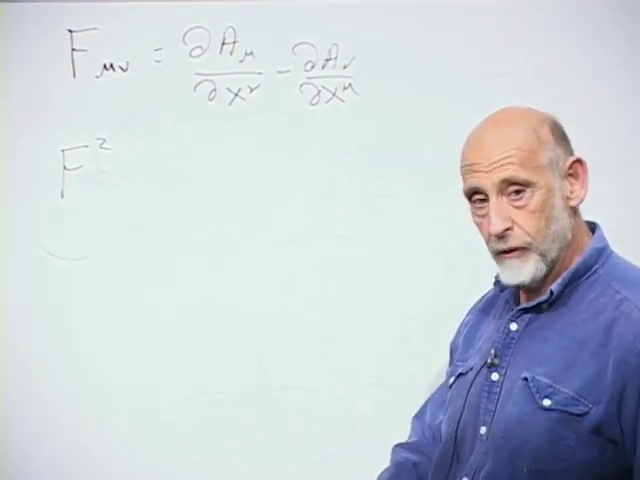
\includegraphics[width=0.72\textwidth]{lecture_09_figure_02.png}
\caption{Định nghĩa cường độ trường và ký hiệu tắt \(F^2\) trên bảng cho năng lượng đạo hàm của trường chuẩn.}
\lectureframe{00:02:39}
\label{fig:l09-field-strength-board}
\end{figure}

Mỗi lần \(A_\mu\) xuất hiện trong \eqref{eq:l09-gauge-kinetic} đều nằm dưới dấu đạo hàm. Vì vậy,
\begin{equation}
  A_\mu(x)\longmapsto A_\mu(x)+c_\mu,
  \qquad \partial_\nu c_\mu=0,
\end{equation}
không làm thay đổi \(F_{\mu\nu}\). Do đó, một thế vectơ đồng nhất không tốn năng lượng cường độ trường. Theo ngôn ngữ của bài giảng, mode xung lượng bằng không không có khe năng lượng và boson chuẩn là không khối lượng.

Trường \(U(1)\) này là một vật thay thế được cố ý làm đơn giản. Đích vật lý thực sự là \(W^\pm\) và \(Z\), chứ không phải photon điện từ. Đối xứng điện từ không bị phá vỡ giữ cho photon không khối lượng; đối xứng điện yếu bị phá vỡ trao khối lượng cho các boson chuẩn yếu.

\subsection{Đóng băng bán kính Higgs}

Hãy đưa vào một trường vô hướng phức mang điện và viết nó ở dạng cực,
\begin{equation}
  \phi(x)=\rho(x)e^{i\alpha(x)}.
\end{equation}
Thế mũ Mexico của nó đạt cực tiểu trên một đường tròn có bán kính khác không. Gọi bán kính ấy là \(f\), thì phương bán kính tương đối cứng. Trong lượt xét đầu tiên, ta đóng băng nó và chỉ giữ lại pha:
\begin{equation}
  \phi(x)\simeq f e^{i\alpha(x)}.
  \label{eq:l09-frozen-higgs}
\end{equation}

\begin{figure}[htbp]
\centering
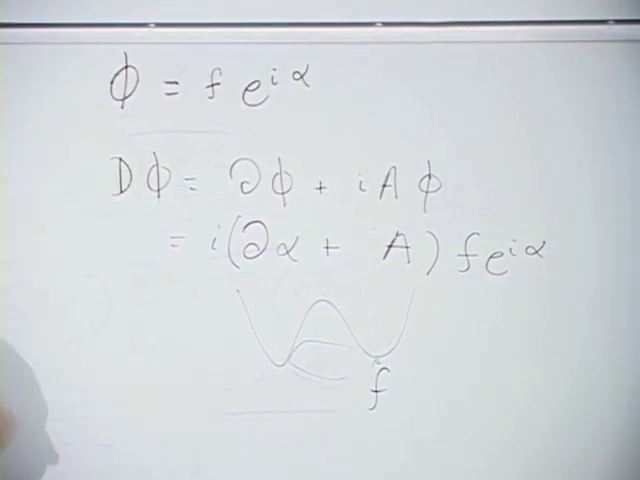
\includegraphics[width=0.72\textwidth]{lecture_09_figure_03.png}
\caption{Bán kính Higgs đã đóng băng, đạo hàm hiệp biến của nó và phác họa nhỏ của thế bị phá vỡ dùng trong phần ôn lại.}
\lectureframe{00:06:42}
\label{fig:l09-frozen-board}
\end{figure}

Chọn quy ước
\begin{equation}
\begin{aligned}
  D_\mu&=\partial_\mu+igA_\mu,
  \\
  \phi&\longmapsto e^{i\theta}\phi,
  \\
  A_\mu&\longmapsto A_\mu-\frac1g\partial_\mu\theta .
\end{aligned}
  \label{eq:l09-gauge-convention}
\end{equation}
Bài giảng ẩn \(g\) đi; giữ nó hiện ra làm cho thứ nguyên và khối lượng xuất hiện về sau trở nên rõ ràng. Tác dụng lên trường đã đóng băng cho
\begin{align}
  D_\mu\phi
  &=(\partial_\mu+igA_\mu)f e^{i\alpha}
  \notag\\
  &=i\bigl(\partial_\mu\alpha+gA_\mu\bigr)
    f e^{i\alpha}.
  \label{eq:l09-covariant-frozen}
\end{align}
Nhân với liên hợp phức loại bỏ pha, đồng thời cũng biến \(i\) nhân \(-i\) thành \(+1\):
\begin{equation}
  |D_\mu\phi|^2
  =f^2
   \bigl(\partial_\mu\alpha+gA_\mu\bigr)
   \bigl(\partial^\mu\alpha+gA^\mu\bigr).
  \label{eq:l09-frozen-square}
\end{equation}

\begin{classroomqa}
\audiencequestion{Bình phương của đạo hàm hiệp biến có nên mang dấu trừ vì đạo hàm tạo ra một thừa số \(i\) không?
\lecturetimestamp{00:07:39}}
\lecturerresponse{Không. Số hạng động học là tích với liên hợp phức. Một thừa số đóng góp \(i\), thừa số kia đóng góp \(-i\), và \(i(-i)=1\). Quy ước dấu cho \(D_\mu\) có thể được đảo một cách nhất quán, nhưng bình phương môđun là dương trong biểu thức năng lượng tương ứng.}
\end{classroomqa}

Tổ hợp trong \eqref{eq:l09-frozen-square} tự nó là một trường chuẩn đã bị dịch. Chọn \(\theta=-\alpha\), để pha của trường vô hướng biến mất, và định nghĩa
\begin{equation}
  A'_\mu=A_\mu+\frac1g\partial_\mu\alpha .
  \label{eq:l09-unitary-gauge-field}
\end{equation}
Khi đó
\begin{equation}
  |D_\mu\phi|^2=g^2f^2 A'_\mu A'^\mu .
  \label{eq:l09-vector-mass-term}
\end{equation}
Số hạng mới không chứa đạo hàm nào của \(A'_\mu\). Bây giờ một trường đồng nhất tích trữ năng lượng, nên mode vectơ xung lượng bằng không có khe năng lượng.

\begin{figure}[htbp]
\centering
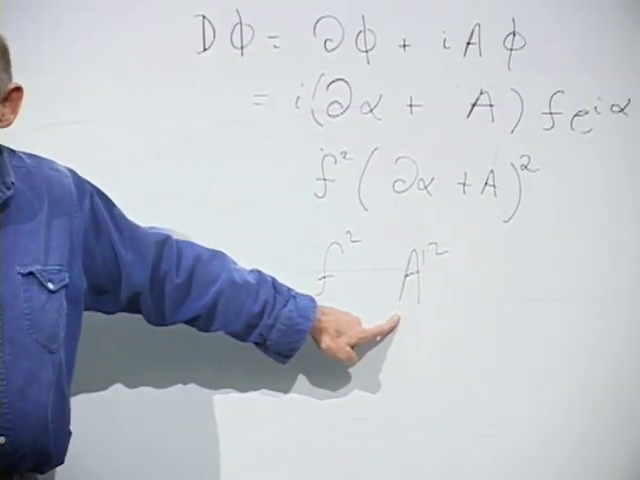
\includegraphics[width=0.72\textwidth]{lecture_09_figure_04.png}
\caption{Trên bảng tách riêng số hạng \(f^2A^2\), báo hiệu khối lượng của boson chuẩn sau khi pha đã được hấp thụ.}
\lectureframe{00:10:31}
\label{fig:l09-vector-mass-board}
\end{figure}

Với chuẩn hóa chuẩn tắc của trường vô hướng, ta viết
\(\phi=(f+h)e^{i\pi/f}/\sqrt2\). So sánh số hạng vectơ thu được với
\(\tfrac12m_A^2A_\mu A^\mu\) cho
\begin{equation}
  m_A=gf
  \label{eq:l09-abelian-vector-mass}
\end{equation}
trong mô hình abel này. Bài giảng ẩn các hệ số chuẩn hóa đi và tóm tắt kết quả bằng cách nói rằng khối lượng vectơ được quyết định bởi \(f\).

Mode pha không biến mất mà không được tính đến. Trước khi đối xứng được chuẩn hóa, nó là một boson Goldstone không khối lượng. Sau khi chuẩn hóa, nó cung cấp phân cực dọc cần thiết cho một hạt vectơ có khối lượng. Dao động theo phương bán kính, thứ mà ta tạm thời đã đóng băng, còn lại như kích thích Higgs vật lý.

\subsection{Vì sao một số hạng không có đạo hàm lại có nghĩa là khối lượng}

\begin{classroomqa}
\audiencequestion{Vì sao một số hạng \(A'^2\) lại được tính là khối lượng chứ không chỉ là một tương tác khác?\lecturetimestamp{00:13:10}}
\lecturerresponse{Khối lượng là năng lượng khi đứng yên. Đối với một trường, một hạt đứng yên là lượng tử của một mode xung lượng bằng không, bước sóng vô hạn. Số hạng đạo hàm không cho năng lượng đối với một độ dời đồng nhất tĩnh, còn \(m_A^2A'^2\) thì có. Năng lượng xung lượng bằng không khác không ấy chính là khe năng lượng nghỉ.}
\end{classroomqa}

Bài giảng triển khai phát biểu này qua ba phép loại suy cơ học.

\begin{itemize}
  \item Trong một tinh thể, một độ dời biến thiên chậm tốn năng lượng đàn hồi vì các nguyên tử lân cận bị dịch đi khác nhau. Một phép tịnh tiến cứng dịch chuyển mọi nguyên tử cùng nhau và không tốn nội năng. Vì vậy phonon âm không có khe năng lượng.
  \item Trong một nam châm lý tưởng đối xứng quay, một phương spin biến thiên theo không gian tốn năng lượng trao đổi, nhưng quay mọi spin cùng nhau thì không. Sóng spin bước sóng dài liên hệ với nó vì thế không có khe năng lượng.
  \item Trong một plasma, dịch chuyển chất lỏng electron so với nền dương tạo ra sự tách điện tích và một điện trường phục hồi ngay cả đối với một độ dời tương đối đồng nhất. Plasmon kết quả có tần số khác không tại số sóng bằng không.
\end{itemize}

Trường chuẩn đã Higgs hóa cư xử giống ví dụ thứ ba: môi trường bị phá vỡ chống lại điều mà nếu không thì sẽ là một độ dời đồng nhất không tốn năng lượng.

\begin{classroomqa}
\audiencequestion{Trước khi đưa trường chuẩn vào, pha \(\alpha\) chẳng phải đã dao động rồi sao?\lecturetimestamp{00:18:24}}
\lecturerresponse{Đúng vậy. Năng lượng của nó tỉ lệ với
\(f^2(\partial_\mu\alpha)^2\). Một pha biến thiên từ nơi này sang nơi khác có năng lượng gradient và có thể lan truyền, nhưng một thay đổi pha đồng nhất thì không tốn gì. Đó chính xác là mode Goldstone không khối lượng.}
\end{classroomqa}

\begin{classroomqa}
\audiencequestion{Đạo hàm có bao gồm đạo hàm theo thời gian. Việc thực sự làm chuyển động cả mạng tinh thể hoặc làm thay đổi toàn bộ trường chẳng phải vẫn mang năng lượng động học sao?\lecturetimestamp{00:22:18}}
\lecturerresponse{Có. Sự so sánh ở đây là giữa các cấu hình tĩnh, hoặc giữa các cấu hình được chuẩn bị chậm tùy ý. Một mạng tinh thể tịnh tiến với vận tốc khác không có năng lượng động học. Phép kiểm tra khối lượng hỏi xem cấu hình ấy có còn năng lượng khi nó đứng yên và đồng nhất trong không gian hay không.}
\end{classroomqa}

\section{Manh mối thực nghiệm: tương tác yếu phân biệt trái và phải}

Bây giờ bài giảng chuyển sang electron, muon và quark. Khối lượng của chúng cũng đến từ trường Higgs, nhưng cơ chế trông khác đi vì khối lượng fermion không phải là một số hạng vectơ bậc hai. Nó là một liên kết giữa hai trường chiral.

\subsection{Vi phạm đối xứng chẵn lẻ trong phân rã beta}

Bắt đầu từ sự kiện thực nghiệm rằng tương tác yếu vi phạm đối xứng chẵn lẻ. Điện động lực học lượng tử và sắc động lực học lượng tử đối xử như nhau với một quá trình và ảnh gương của nó. Tương tác yếu thì không. Trong phân rã beta của neutron,
\begin{equation}
  n\longrightarrow p+e^-+\bar\nu_e,
  \label{eq:l09-beta-decay}
\end{equation}
những electron năng lượng cao được tương tác dòng mang điện chọn lọc có helicity trái: spin của chúng hướng ngược với xung lượng. Các phản neutrino tương ứng có helicity ngược lại.

Đối với một hạt siêu tương đối tính, định nghĩa helicity bằng
\begin{equation}
  h=\frac{\bm S\cdot\bm p}{|\bm S|\,|\bm p|}.
\end{equation}
Spin song song với xung lượng có \(h=+1\); spin ngược song song có \(h=-1\). Tương tác yếu ghép với một trường electron chiral trái và một trường neutrino chiral trái, chứ không ghép với một trường electron chiral phải theo cùng cách đó.\editorialnote{Ban đầu bài giảng dùng tính tay theo nghĩa helicity vì điều đó trực quan về mặt hình dung ở năng lượng cao. Các điện tích chuẩn thực sự tác dụng lên chirality, nhãn biểu diễn Lorentz được chọn bởi \(P_L=(1-\gamma^5)/2\) và \(P_R=(1+\gamma^5)/2\). Đối với một hạt không khối lượng, chirality và helicity trùng nhau đối với hạt; đối với một hạt có khối lượng thì chúng không trùng nhau.}

Để làm lộ ra chướng ngại này mà không cần toàn bộ phần hạch toán \(SU(2)_L\times U(1)_Y\), hãy tưởng tượng một thế giới \(U(1)\) giả trong đó chỉ \(\psi_L\) mang điện tích liên quan:
\begin{equation}
  \psi_L\longmapsto e^{i\theta}\psi_L,
  \qquad
  \psi_R\longmapsto\psi_R .
  \label{eq:l09-chiral-toy-charge}
\end{equation}
Đây không phải điện từ học: các electron chiral trái và chiral phải thực sự mang cùng điện tích điện. Nó là một bức biếm họa của tương tác yếu, trong đó hai chirality nằm trong các biểu diễn điện yếu khác nhau.

\begin{classroomqa}
\audiencequestion{Sự bất đối xứng trái--phải ấy có áp dụng tương tự cho quark không?
\lecturetimestamp{00:31:50}}
\lecturerresponse{Có, với các đa tuyến yếu và hypercharge thích hợp. Các quark chiral trái kiểu up và kiểu down tạo thành các doublet yếu, còn các trường chiral phải là các singlet yếu. Vì vậy, các liên kết Higgs của chúng cũng đối mặt với cùng một vấn đề cấu trúc như của electron.}
\end{classroomqa}

\section{Khối lượng Dirac là sự trộn trái--phải}

\subsection{Từ phương trình bốn thành phần đến hai phương trình Weyl}

Một hàm sóng Dirac có bốn thành phần. Nói một cách lỏng lẻo, hai thành phần mô tả spin và hai thành phần phân biệt các nghiệm năng lượng dương và năng lượng âm, trong đó các nghiệm sau được diễn giải lại như các bậc tự do phản hạt. Ở dạng Hamilton,
\begin{equation}
  i\frac{\partial\Psi}{\partial t}
  =\left(-i\bm\alpha\cdot\bm\nabla+m\beta\right)\Psi .
  \label{eq:l09-dirac-hamiltonian}
\end{equation}
Các ma trận \(\alpha_i\) và \(\beta\) mã hóa quan hệ tương đối tính giữa năng lượng, xung lượng và khối lượng.

\begin{figure}[htbp]
\centering
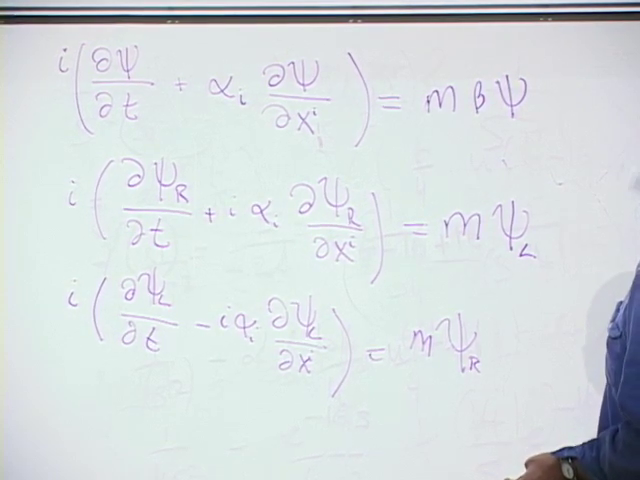
\includegraphics[width=0.74\textwidth]{lecture_09_figure_05.png}
\caption{Trên bảng trước hết viết phương trình Dirac, rồi tách nó thành các phương trình tay trái và tay phải ghép cặp với nhau.}
\lectureframe{00:40:30}
\label{fig:l09-dirac-board}
\end{figure}

Cơ sở chiral làm cho vai trò của \(m\) trở nên tường minh. Với
\(\sigma^\mu=(1,\bm\sigma)\) và
\(\bar\sigma^\mu=(1,-\bm\sigma)\),
\begin{align}
  i\bar\sigma^\mu\partial_\mu\psi_L&=m\psi_R,
  \label{eq:l09-weyl-left}\\
  i\sigma^\mu\partial_\mu\psi_R&=m\psi_L.
  \label{eq:l09-weyl-right}
\end{align}
Khi \(m=0\), các phương trình độc lập: một trường chiral trái và một trường chiral phải có thể lan truyền mà không ghép với nhau. Khi \(m\neq0\), mỗi trường xuất hiện như nguồn của trường kia. Đó là nghĩa chính xác mà theo đó một khối lượng Dirac trộn trái và phải.

Susskind mô tả điều này như fermion dao động giữa trái và phải. Lối nói ấy nắm bắt được sự ghép, nhưng không nên đẩy nó thành một bức tranh cổ điển theo nghĩa đen về một hạt điểm lật qua lật lại. Phát biểu chính xác là hệ phương trình trường ghép
\eqref{eq:l09-weyl-left}--\eqref{eq:l09-weyl-right}.

\begin{classroomqa}
\audiencequestion{Các thừa số \(i\) và các dấu trong hai phương trình trên bảng có nhất quán không?\lecturetimestamp{00:41:10}}
\lecturerresponse{Nếu xét từng dòng trên bảng thì không; một \(i\) đã bị kéo ra ngoài một cách không nhất quán trong phép suy ra nhanh. Nội dung đáng tin cậy là mô thức ghép. Các phương trình \eqref{eq:l09-weyl-left} và
\eqref{eq:l09-weyl-right} cho một quy ước nhất quán tiêu chuẩn.}
\end{classroomqa}

\subsection{Vì sao đối xứng yếu cấm một khối lượng trần}

Số hạng khối lượng Dirac tương ứng trong Lagrangian là
\begin{equation}
  \mathcal L_m
  =-m\bar\psi\psi
  =-m\left(\bar\psi_L\psi_R+\bar\psi_R\psi_L\right).
  \label{eq:l09-bare-dirac-mass}
\end{equation}
Dưới phép biến đổi mô hình đồ chơi \eqref{eq:l09-chiral-toy-charge},
\begin{equation}
  \bar\psi_L\psi_R\longmapsto
  e^{-i\theta}\bar\psi_L\psi_R,
  \qquad
  \bar\psi_R\psi_L\longmapsto
  e^{i\theta}\bar\psi_R\psi_L.
\end{equation}
Không số hạng nào là bất biến. Vì vậy hệ số trộn trực tiếp trái--phải \(m\) bị cấm trước khi đối xứng bị phá vỡ.

Chỉ riêng điện từ học sẽ không gây ra vấn đề này, vì \(\psi_L\) và
\(\psi_R\) có cùng điện tích điện. Chướng ngại nảy sinh từ các số lượng tử yếu khác nhau của chúng.

\subsection{Các câu hỏi về helicity làm lộ ra sự tinh tế của chirality}

Bây giờ lớp học kiểm tra bức tranh trực giác về tính tay từ nhiều góc độ. Những câu hỏi này không phải chuyện bên lề: chúng chỉ ra chính xác helicity hữu ích ở đâu và ở đâu chirality phải thay thế nó.

\begin{classroomqa}
\audiencequestion{Thế giới sẽ ra sao nếu tương tác yếu phát ra electron với cả hai độ xoắn như nhau?\lecturetimestamp{00:42:12}}
\lecturerresponse{Sự bất đối xứng chẵn lẻ trực tiếp sẽ biến mất khỏi quá trình đó. Nhưng lý thuyết điện yếu thực sự là chiral: chỉ các bộ đôi chiral trái mới mang tương tác yếu mang điện. Bài giảng tạm hoãn một trình bày đầy đủ hơn về vì sao tự nhiên lại chọn cấu trúc đó.}
\end{classroomqa}

\begin{classroomqa}
\audiencequestion{Giả sử spin của một electron được chuẩn bị theo phương thẳng đứng và sau đó electron được gia tốc theo phương ngang. Nó là tay trái hay tay phải?
\lecturetimestamp{00:42:44}}
\lecturerresponse{Một trạng thái spin vuông góc với động lượng là chồng chập của hai độ xoắn. Độ xoắn chỉ xác định rõ khi spin song song hoặc phản song song với động lượng. Tuy vậy, các toán tử chiếu chiral yếu vẫn được xác định rõ cho trường.}
\end{classroomqa}

Một hạt có khối lượng có thể bị làm chậm đến đứng yên rồi được gia tốc theo hướng ngược lại mà không đảo spin của nó. Khi đó độ xoắn của nó đổi dấu. Một hạt không khối lượng không thể bị vượt qua hoặc bị đưa về trạng thái đứng yên bằng một phép boost Lorentz, nên độ xoắn của nó bất biến dưới các phép boost Lorentz riêng. Điều này thúc đẩy phát biểu trong bài giảng rằng một loại hạt chỉ có một độ xoắn vật lý thì phải không khối lượng. Phát biểu chính xác hơn trong lý thuyết trường là một hạng khối lượng Dirac bất biến Lorentz đòi hỏi cả hai thành phần chiral.

\begin{classroomqa}
\audiencequestion{Một photon phân cực tròn có thể phản xạ trên gương và đảo hướng mà không hề dừng lại. Điều đó có mâu thuẫn với lập luận về độ xoắn không?\lecturetimestamp{00:45:28}}
\lecturerresponse{Không. Gương là một hệ bên ngoài có thể trao đổi mômen góc và đảo hướng lan truyền. Một quá trình phản xạ không phải là một phép boost Lorentz vượt qua photon. Việc có tồn tại một kênh hay không còn phụ thuộc vào các trạng thái phân cực được phép và các điều kiện biên của vật liệu.}
\end{classroomqa}

\begin{classroomqa}
\audiencequestion{Một chùm electron thông thường chứa chỉ một loại thuận tay hay cả hai?\lecturetimestamp{00:46:10}}
\lecturerresponse{Nói chung là cả hai. Một trạng thái electron có khối lượng chứa cả hai thành phần chiral, và một chùm không phân cực chứa cả hai độ xoắn. Các nguồn chuyên dụng có thể tạo ra một chùm phân cực với bất đối xứng độ xoắn lớn.}
\end{classroomqa}

\begin{classroomqa}
\audiencequestion{Có thể hội tụ một chùm độc lập với spin của nó không, hay từ trường tách hai phân cực ra?\lecturetimestamp{00:46:29}}
\lecturerresponse{Việc hội tụ vị trí thông thường có thể phần lớn không nhạy với spin, nhưng mômen từ lại ghép với gradient từ trường. Vì vậy, các nguồn chọn lọc spin, các gradient kiểu Stern--Gerlach, và động lực học spin trong máy gia tốc có thể chuẩn bị hoặc tách các phân cực.}
\end{classroomqa}

\begin{classroomqa}
\audiencequestion{Sự khác biệt trong tương tác yếu giữa trái và phải có chỉ là ngẫu nhiên không?\lecturetimestamp{00:48:13}}
\lecturerresponse{Đối với học phần hiện tại, đó là một sự kiện thực nghiệm đã được đưa vào Mô hình Chuẩn. Nó quá có hệ thống để có cảm giác như một sự tình cờ đơn thuần, nhưng bản thân Mô hình Chuẩn không suy ra mẫu đầy đủ của các điện tích chiral từ một nguyên lý sâu hơn.}
\end{classroomqa}

\section{Xây dựng Yukawa}

\subsection{Để Higgs mang điện tích còn thiếu}

Đối xứng cấm một hạng khối lượng dạng số, nhưng nó cho phép một tương tác với một trường cung cấp pha biến đổi còn thiếu. Hãy đưa vào một trường vô hướng phức với
\begin{equation}
  \phi\longmapsto e^{i\theta}\phi,
  \qquad
  \phi^\dagger\longmapsto e^{-i\theta}\phi^\dagger.
  \label{eq:l09-scalar-charge}
\end{equation}
Khi đó
\begin{equation}
  \mathcal L_Y
  =-y\,\bar\psi_L\phi\psi_R
   -y^*\,\bar\psi_R\phi^\dagger\psi_L
  \label{eq:l09-yukawa-lagrangian}
\end{equation}
là bất biến chuẩn. Trong hạng thứ nhất,
\(\bar\psi_L\) đóng góp \(e^{-i\theta}\) và \(\phi\) đóng góp
\(e^{i\theta}\); các pha triệt tiêu nhau. Hạng thứ hai là liên hợp Hermite của hạng đó.

Tương đương, các phương trình chiral thu được sự trộn phụ thuộc vào trường:
\begin{align}
  i\bar\sigma^\mu D_\mu\psi_L
    &=y\phi\psi_R,
  \label{eq:l09-yukawa-eom-left}\\
  i\sigma^\mu\partial_\mu\psi_R
    &=y^*\phi^\dagger\psi_L.
  \label{eq:l09-yukawa-eom-right}
\end{align}

\begin{figure}[htbp]
\centering
\includegraphics[width=0.76\textwidth]{lecture_09_figure_06.png}
\caption{Khối lượng trần ở các vế phải đã được thay bằng trường vô hướng mang điện. Các dấu viết trên bảng chỉ có tính sơ đồ; cấu trúc bất biến được cho trong \eqref{eq:l09-yukawa-lagrangian}.}
\lectureframe{00:51:30}
\label{fig:l09-yukawa-board}
\end{figure}

Trước khi đối xứng bị phá vỡ, đây là một tương tác chứ không phải khối lượng. Một fermion chiral phải chỉ có thể trở thành một fermion chiral trái khi phát ra hoặc hấp thụ lượng tử của trường vô hướng cần thiết để cân bằng điện tích. Hệ số \(y\) là hằng số ghép Yukawa, không phải điện tích chuẩn \(g\).

\begin{classroomqa}
\audiencequestion{Có hợp lệ không nếu đơn giản đặt \(\phi\) và
\(\phi^\dagger\) vào vế phải của hai phương trình?
\lecturetimestamp{00:51:55}}
\lecturerresponse{Điều đó hợp lệ chính vì các pha biến đổi của chúng sửa chữa sự không khớp. Phép kiểm tra quyết định không phải là hình thức bề ngoài của phương trình mà là tính bất biến chuẩn của tương tác
\(\bar\psi_L\phi\psi_R+\mathrm{h.c.}\).}
\end{classroomqa}

\subsection{Chân không biến tương tác thành khối lượng}

Bây giờ hãy đồng nhất \(\phi\) với trường Higgs và cho nó ổn định ở một độ lớn chân không khác không. Theo chuẩn hoá đơn giản hoá của bài giảng,
\begin{equation}
  \phi\simeq f,
\end{equation}
nên \eqref{eq:l09-yukawa-lagrangian} chứa
\begin{equation}
  \mathcal L_Y
  \supset
  -yf\,\bar\psi_L\psi_R
  -y^*f\,\bar\psi_R\psi_L .
\end{equation}
Sau một phép tái định nghĩa pha vô hại, khi thích hợp, khối lượng fermion là
\begin{equation}
  m_f=yf.
  \label{eq:l09-lecture-fermion-mass}
\end{equation}
Đây là đối ứng fermion của kết quả vectơ \(m_A=gf\). Cùng một chân không Higgs vừa cung cấp một phân cực dọc cho các boson chuẩn yếu vừa cung cấp các số lượng tử yếu còn thiếu cần thiết để ghép các fermion trái và phải.

Trong quy ước Mô hình Chuẩn với chuẩn hoá chính tắc,
\begin{equation}
  H(x)=\frac1{\sqrt2}
  \begin{pmatrix}
    0\\ v+h(x)
  \end{pmatrix},
  \qquad v\simeq246\ \mathrm{GeV},
  \label{eq:l09-sm-higgs-vacuum}
\end{equation}
và do đó
\begin{equation}
  m_f=\frac{y_fv}{\sqrt2}.
  \label{eq:l09-sm-fermion-mass}
\end{equation}
\(f\) của bài giảng và \(v/\sqrt2\) theo quy ước chỉ khác nhau bởi lựa chọn chuẩn hoá này.

\begin{classroomqa}
\audiencequestion{Nếu chỉ tích \(yf\) mới là khối lượng fermion, thì làm sao có thể xác định riêng rẽ hằng số ghép \(y\) và thang chân không \(f\)?
\lecturetimestamp{00:55:36}}
\lecturerresponse{Khối lượng của các boson chuẩn yếu xác định thang chân không một khi các hằng số ghép chuẩn đã biết. Khi đó khối lượng đo được của một fermion xác định hằng số ghép Yukawa của nó. Trong lý thuyết đầy đủ,
\(m_W=gv/2\), \(m_Z=v\sqrt{g^2+g'^2}/2\), và
\(y_f=\sqrt2m_f/v\).}
\end{classroomqa}

\begin{classroomqa}
\audiencequestion{Khối lượng boson yếu có khoảng \(900\ \mathrm{GeV}\) không?
\lecturetimestamp{00:57:43}}
\lecturerresponse{Không; bài giảng ngay lập tức sửa chỗ lỡ lời đó thành xấp xỉ
\(90\ \mathrm{GeV}\). Chính xác hơn,
\(m_W\simeq80\ \mathrm{GeV}\) và \(m_Z\simeq91\ \mathrm{GeV}\), trong khi thang chân không nền tảng là \(v\simeq246\ \mathrm{GeV}\).}
\end{classroomqa}

\subsection{Một thang chân không, nhiều hằng số ghép Yukawa}

Mỗi loài fermion mang điện có hằng số ghép Yukawa riêng:
\begin{equation}
  m_i=y_i f
  \qquad\text{(lecture normalization)}.
  \label{eq:l09-mass-family}
\end{equation}

\begin{figure}[htbp]
\centering
\includegraphics[width=0.76\textwidth]{lecture_09_figure_08.png}
\caption{Trên bảng, sự phụ thuộc theo loài được tóm tắt thành \(m_i=g_i f\); các \(g_i\) viết ở đó chính là các hằng số ghép Yukawa được gọi là \(y_i\) ở đây.}
\lectureframe{01:16:30}
\label{fig:l09-mass-family-board}
\end{figure}

Đối với electron, bài giảng ước lượng
\begin{equation}
  y_e\sim\frac{0.5\ \mathrm{MeV}}{10^2\ \mathrm{GeV}}
  \sim10^{-5}.
\end{equation}
Dùng giá trị chính tắc \(v=246\ \mathrm{GeV}\) cho kết quả chính xác hơn là
\(y_e\simeq2.9\times10^{-6}\). Quark top nằm ở đầu đối diện:
\begin{equation}
  y_t=\frac{\sqrt2m_t}{v}\simeq1.
\end{equation}
Vì vậy, cơ chế Higgs giải thích bằng cách nào một khối lượng bất biến chuẩn có thể tồn tại, nhưng nó không giải thích được thứ bậc cực lớn giữa các \(y_i\). Các khối lượng fermion quan sát được chỉ đơn thuần chuyển thứ bậc đó thành các con số đo được.

\begin{classroomqa}
\audiencequestion{Quark top thực sự có hằng số ghép Yukawa cỡ 1 sao?\lecturetimestamp{00:59:09}}
\lecturerresponse{Có. Khối lượng của nó so sánh được với thang điện yếu, nên hằng số ghép của nó không phải là một số nhiễu loạn rất nhỏ như của electron. Trong chuẩn hoá hiện đại, \(y_t\) gần bằng 1.}
\end{classroomqa}

\subsection{Khôi phục dao động Higgs vật lý}

Việc giữ cố định trường vô hướng ở giá trị chân không của nó đã che khuất kích thích hướng xuyên tâm. Khôi phục nó một cách sơ đồ:
\begin{equation}
  \phi(x)\simeq f+h(x).
\end{equation}
Thừa số Yukawa trở thành
\begin{equation}
  y\phi\simeq yf+yh=m_f+yh.
  \label{eq:l09-mass-plus-higgs}
\end{equation}

\begin{figure}[htbp]
\centering
\includegraphics[width=0.76\textwidth]{lecture_09_figure_07.png}
\caption{Trên bảng, dao động Higgs được khôi phục bên trong hạng Yukawa: phần hằng sinh ra khối lượng fermion và phần dao động sinh ra sự phát xạ hoặc hấp thụ Higgs.}
\lectureframe{01:01:15}
\label{fig:l09-higgs-fluctuation-board}
\end{figure}

Hạng thứ nhất trong \eqref{eq:l09-mass-plus-higgs} là khối lượng. Hạng thứ hai là một đỉnh trong đó một boson Higgs ghép với fermion. Trong ký hiệu Mô hình Chuẩn chuẩn hoá chính tắc,
\begin{equation}
  \mathcal L_Y
  \supset
  -m_f\bar\psi\psi
  -\frac{m_f}{v}h\bar\psi\psi.
  \label{eq:l09-higgs-fermion-vertex}
\end{equation}
Hằng số ghép tỉ lệ với khối lượng fermion. Có tính đến động học, các hệ số màu, không gian pha và các kênh cạnh tranh, vì vậy Higgs ghép mạnh hơn với các fermion nặng hơn.

\begin{classroomqa}
\audiencequestion{Bản thân các hằng số ghép có phải là xác suất không?
\lecturetimestamp{01:03:35}}
\lecturerresponse{Chúng đi vào các biên độ lượng tử. Một tốc độ đơn giản thường tỉ lệ với bình phương môđun của một biên độ và do đó với bình phương hằng số ghép, nhưng không gian pha, tổng spin, giao thoa, các vòng, và nhiều đỉnh cũng đều quan trọng. Không nên đồng nhất trực tiếp một hằng số ghép với xác suất.}
\end{classroomqa}

\begin{classroomqa}
\audiencequestion{Lập luận này có giả sử chỉ có một trường Higgs không?\lecturetimestamp{01:03:59}}
\lecturerresponse{Nó mô tả Mô hình Chuẩn tối thiểu, vốn có một bộ đôi Higgs phức. Ba trong bốn thành phần thực của nó bị hấp thụ bởi \(W^\pm\) và \(Z\), để lại một vô hướng trung hoà vật lý. Các mở rộng có thể chứa nhiều bộ đôi hơn hoặc các đa bội vô hướng khác. Các mô hình siêu đối xứng thường đòi hỏi hai bộ đôi Higgs và do đó chứa một số trạng thái Higgs vật lý.}
\end{classroomqa}

Kỳ vọng lịch sử đó nay có thể được so sánh với thực nghiệm.
\editorialnote{Bài giảng này được ghi lại trước khi Higgs được phát hiện. ATLAS và CMS công bố một hạt giống Higgs vào 2012, hiện được đo gần \(125\ \mathrm{GeV}\). Các hằng số ghép quan sát được của nó nhìn chung phù hợp với khuôn mẫu Mô hình Chuẩn tỉ lệ theo khối lượng. Phát biểu rằng nó phân rã ưu tiên thành các hạt nặng nhất luôn kèm theo lưu ý động học: một cặp \(t\bar t\) trên vỏ quá nặng đối với một Higgs \(125\ \mathrm{GeV}\).}

\section{Phản hạt, chùm hạt và ý nghĩa của tính chiral}

Trước khi chuyển sang neutrino, lớp quay lại một số câu hỏi thực hành về phản hạt và các chùm hạt trong máy gia tốc.

\begin{classroomqa}
\audiencequestion{Phản hạt của một electron tay trái có tính tay gì?\lecturetimestamp{01:06:05}}
\lecturerresponse{Một trường electron chiral trái hủy các electron có helicity trái và tạo các positron có helicity phải trong giới hạn siêu tương đối tính. Đây là một chỗ mà sự phân biệt giữa hạt với phản hạt và giữa chiral với helicity phải được nêu thật cẩn thận.}
\end{classroomqa}

\begin{classroomqa}
\audiencequestion{Electron và positron có thể va chạm để tạo ra một boson \(Z\) không?\lecturetimestamp{01:07:13}}
\lecturerresponse{Có, khi năng lượng khối tâm của chúng khớp với kênh được phép. Các máy va chạm electron--positron đã nghiên cứu cộng hưởng \(Z\) với độ chính xác rất cao. Điện tích và các số lượng tử khác được bảo toàn trong toàn bộ quá trình.}
\end{classroomqa}

\begin{classroomqa}
\audiencequestion{Có phải mọi positron đều được tạo ra thông qua một quá trình yếu đặc biệt không?\lecturetimestamp{01:07:37}}
\lecturerresponse{Không. Tạo cặp là một con đường điện từ thông thường. Ví dụ, một electron năng lượng cao có thể bức xạ một photon ảo, và photon đó có thể tạo ra một cặp \(e^-e^+\) trong trường của một hạt khác. Bài giảng phác hoạ điều này bằng một giản đồ Feynman.}
\end{classroomqa}

\begin{classroomqa}
\audiencequestion{Một máy gia tốc thẳng có thể chọn tốc độ hay năng lượng của electron không?\lecturetimestamp{01:09:24}}
\lecturerresponse{Có. Các trường gia tốc và thời điểm đồng bộ chọn ra một khoảng năng lượng. Một khi electron đã siêu tương đối tính thì tốc độ của chúng vốn đã cực kỳ gần \(c\), nên năng lượng bổ sung từ máy gia tốc chủ yếu làm tăng động lượng và tổng năng lượng hơn là làm tăng tốc độ một cách thấy rõ.}
\end{classroomqa}

\begin{classroomqa}
\audiencequestion{Một máy gia tốc có thể chuẩn bị một chùm với một phân cực duy nhất không?
\lecturetimestamp{01:09:47}}
\lecturerresponse{Có, mặc dù đòi hỏi kỹ thuật cao. Người ta có thể chuẩn bị các electron phân cực spin ở năng lượng thấp bằng một nguồn phụ thuộc spin rồi gia tốc chúng trong khi kiểm soát sự tiến động spin. Các máy va chạm hiện đại định lượng độ phân cực chùm thu được thay vì coi nó là tinh khiết hoàn toàn.}
\end{classroomqa}

\section{Khối lượng neutrino và khả năng Majorana}

\subsection{Vì sao khối lượng neutrino buộc phải mở rộng lý thuyết}

Mô hình Chuẩn tối thiểu ban đầu chỉ bao gồm các trường neutrino chiral trái và vì thế dự đoán neutrino không có khối lượng. Dao động neutrino cho thấy ít nhất hai trị riêng khối lượng neutrino là khác nhau và rằng khối lượng neutrino khác không, dù rất nhỏ so với khối lượng của các fermion mang điện.

\begin{classroomqa}
\audiencequestion{Khối lượng neutrino nhỏ đến mức nào, và thành phần chiral phải của chúng ở đâu?\lecturetimestamp{01:10:38}}
\lecturerresponse{Dao động xác định các hiệu bình phương khối lượng, chứ không xác định các khối lượng tuyệt đối. Các độ tách liên quan tương ứng với những thang cỡ khoảng \(0.009\ \mathrm{eV}\) và \(0.05\ \mathrm{eV}\). Một mô tả Dirac thêm các neutrino chiral phải vô sinh; còn mô tả Majorana thì thay vào đó liên hệ thành phần chiral còn thiếu với các trường neutrino liên hợp điện tích.}
\end{classroomqa}

Đối với neutrino Dirac, ta thêm một trường mới \(\nu_R\) và lặp lại phép xây dựng Yukawa:
\begin{equation}
  \mathcal L_{\nu,\mathrm{Dirac}}
  =-y_\nu\bar L\,\widetilde H\,\nu_R+\mathrm{h.c.},
  \qquad
  m_\nu=\frac{y_\nu v}{\sqrt2}.
  \label{eq:l09-dirac-neutrino}
\end{equation}
Giá trị \(y_\nu\) cần thiết là cực kỳ nhỏ.

Có một khả năng logic khác vì neutrino không mang điện tích điện. Một neutrino chiral trái có thể được ghép với liên hợp điện tích của chính nó, đối tượng này có chirality ngược lại:
\begin{equation}
  \nu_L\longleftrightarrow(\nu_L)^c_R .
  \label{eq:l09-majorana-mixing}
\end{equation}
Một trạng thái riêng khối lượng được xây dựng theo cách này là một fermion Majorana: nó là phản hạt của chính nó, ngoại trừ các quy ước pha. Sự trộn electron--positron tương tự bị cấm vì nó sẽ vi phạm sự bảo toàn điện tích điện chính xác.

\begin{classroomqa}
\audiencequestion{Vì sao sự trộn hạt--phản hạt được phép đối với neutrino nhưng không đối với electron?\lecturetimestamp{01:13:43}}
\lecturerresponse{Electron và positron có điện tích điện trái dấu, nên một hạng khối lượng trộn chúng thành cùng một trạng thái một hạt sẽ vi phạm đối xứng điện từ không bị phá vỡ. Neutrino thì trung hòa điện. Nếu không có số lepton bảo toàn chính xác nào phân biệt nó với phản hạt của nó, thì một khối lượng Majorana được phép.}
\end{classroomqa}

Tên gọi này nhằm vinh danh Ettore Majorana, nhà vật lý Ý trẻ tuổi đã xây dựng kiểu biểu diễn fermion thực này và biến mất vào 1938. Bài giảng dừng lại ở bí ẩn lịch sử ấy: số phận của ông chưa bao giờ được xác định. \editorialnote{Một khối lượng Majorana bất biến chuẩn cho neutrino hoạt động của Mô hình Chuẩn không phải là một hạng trần khả tái chuẩn hóa trước khi đối xứng điện yếu bị phá vỡ. Ở năng lượng thấp, nó có thể phát sinh từ toán tử Weinberg bậc năm \((LH)(LH)/\Lambda\), hoặc thông qua một cơ chế seesaw có sự tham gia của các neutrino vô sinh nặng. Việc neutrino là hạt Dirac hay Majorana vẫn chưa được thực nghiệm phân định.}

\section{Vì sao phổ quen thuộc lại tụ gần thang điện yếu}

\subsection{Thang chung và những lưu ý quan trọng kèm theo}

\begin{classroomqa}
\audiencequestion{Vì sao khối lượng Higgs được kỳ vọng là nằm trong tầm với ở thang yếu?\lecturetimestamp{01:14:48}}
\lecturerresponse{Độ cong của thế Higgs ấn định khối lượng Higgs theo phương xuyên tâm, trong khi cùng thang chân không \(f\) ấn định các khối lượng của \(W\) và \(Z\). Vì thế, nếu không có tự liên kết vô hướng cực đoan, người ta kỳ vọng khối lượng Higgs có cùng bậc độ lớn tổng quát với thang yếu. Giá trị quan sát được \(125\ \mathrm{GeV}\) quả thực nằm ở đó.}
\end{classroomqa}

Tóm tắt nổi bật của bài giảng là các khối lượng sơ cấp của Mô hình Chuẩn tối thiểu đều bắt nguồn từ một chân không bị phá vỡ:
\begin{align}
  m_W&=\frac12gv,\\
  m_Z&=\frac12\sqrt{g^2+g'^2}\,v,\\
  m_f&=\frac1{\sqrt2}y_fv.
  \label{eq:l09-electroweak-mass-summary}
\end{align}
Nếu \(v\) bằng không trong khi các hằng số ghép không thứ nguyên được giữ cố định, thì các boson chuẩn yếu và các fermion sơ cấp mang điện sẽ không có khối lượng.

Mệnh đề ấy không được mở rộng ra ngoài phạm vi của nó. Photon và gluon vẫn không có khối lượng vì một đối xứng chuẩn không bị phá vỡ bảo vệ chúng. Phần lớn khối lượng của proton và neutron là năng lượng liên kết QCD, chứ không phải tổng các khối lượng Higgs của các quark cấu thành chúng. Khối lượng neutrino đòi hỏi một mở rộng của mô hình tối thiểu. Bản thân khối lượng Higgs phụ thuộc vào thế vô hướng và không đơn giản chỉ là một khối lượng Yukawa khác.

\subsection{Những hạt có khối lượng không nhất thiết phải chờ sự phá vỡ đối xứng}

Giả sử một fermion mới có các thành phần chiral trái và chiral phải với các số lượng tử chuẩn giống hệt nhau. Khi đó \(\bar\Psi_L\Psi_R+\mathrm{h.c.}\) đã là bất biến chuẩn. Một fermion \emph{kiểu vectơ} như vậy có thể có một khối lượng trần \(M\) không liên hệ với \(v\):
\begin{equation}
  \mathcal L_{\mathrm{vectorlike}}
  =-M\bar\Psi\Psi.
  \label{eq:l09-vectorlike-mass}
\end{equation}
Không có sự cản trở nào từ đối xứng điện yếu đối với \(M\gg v\).

Điều này thúc đẩy lập luận rộng về tính tự nhiên của bài giảng. Những hạt được bảo vệ bởi đối xứng chuẩn hoặc đối xứng chiral vẫn không có khối lượng cho đến khi chân không Higgs phá vỡ sự bảo vệ đó, nên khối lượng của chúng gắn với thang tương đối nhỏ \(v\). Những hạt không có sự bảo vệ như vậy một cách tự nhiên có thể nặng hơn nhiều và do đó vắng mặt khỏi phổ năng lượng thấp quan sát được. Cái chúng ta thấy có thể là một hiệu ứng chọn lọc: các hạt có thể tiếp cận được là những hạt mà khối lượng của chúng buộc phải chờ sự phá vỡ đối xứng điện yếu.

\begin{classroomqa}
\audiencequestion{Liệu các hạt có những khối lượng độc lập và lớn hơn nhiều sẽ không đóng vai trò nào trong thực tế sao?\lecturetimestamp{01:19:39}}
\lecturerresponse{Chúng sẽ đóng vai trò nhỏ trong vật lý phòng thí nghiệm năng lượng thấp thông thường vì khó tạo ra chúng, nhưng chúng vẫn có thể định hình lịch sử năng lượng cao hoặc vũ trụ học. Bài giảng nêu vật chất tối như một nơi khả dĩ mà ở đó một phổ ẩn nặng hơn có thể tự bộc lộ lần đầu.}
\end{classroomqa}

Phần thảo luận năm 2010 phản ánh kỳ vọng khi đó đang thịnh hành về vật chất tối ở thang yếu hoặc hơi nặng hơn. Đó vẫn là một lớp mô hình hữu ích, không phải một sự kiện đã được xác lập. Vật chất tối đã được phát hiện qua hấp dẫn, nhưng bản dạng hạt của nó và nguồn gốc khối lượng của nó vẫn chưa được biết.

\section{Các câu hỏi kết thúc: tia vũ trụ, quán tính, hấp dẫn và tính chiral}

\subsection{Khối lượng không đồng nghĩa với năng lượng phòng thí nghiệm cao}

\begin{classroomqa}
\audiencequestion{Khối lượng của một tia vũ trụ là gì?
\lecturetimestamp{01:20:57}}
\lecturerresponse{Một tia vũ trụ có thể là proton, hạt nhân nguyên tử, electron hoặc photon; khối lượng bất biến của nó là khối lượng của hạt hoặc hệ đó. Điều nổi bật là năng lượng của nó trong hệ phòng thí nghiệm, mà đối với các sự kiện cao nhất đạt xấp xỉ từ \(10^{20}\) đến \(10^{21}\ \mathrm{eV}\). Năng lượng cao không đồng nghĩa với khối lượng bất biến lớn.}
\end{classroomqa}

Một tia vũ trụ đập vào một hạt bia gần như đứng yên. Với một proton tới có năng lượng phòng thí nghiệm \(E\gg m_p\),
\begin{equation}
  s=(p_1+p_2)^2
  \simeq2m_pE+2m_p^2,
  \qquad
  \sqrt{s}\simeq\sqrt{2m_pE}.
  \label{eq:l09-fixed-target-s}
\end{equation}
Chỉ căn bậc hai của năng lượng hạt tới trở thành năng lượng khối tâm. Với hai chùm đối đầu có năng lượng bằng nhau \(E_{\rm beam}\),
\begin{equation}
  \sqrt{s}\simeq2E_{\rm beam}.
  \label{eq:l09-collider-s}
\end{equation}
Đó là lý do vì sao máy va chạm hiệu quả hơn rất nhiều so với bia cố định trong việc chuyển năng lượng chùm được kiểm soát thành khối lượng của hạt mới.

\begin{classroomqa}
\audiencequestion{Vì sao máy va chạm của CERN có thể là một đầu dò mạnh hơn so với một hạt đơn lẻ có năng lượng lớn hơn nhiều đập vào vật chất đứng yên?
\lecturetimestamp{01:21:50}}
\lecturerresponse{Trong va chạm bia cố định, bảo toàn động lượng mang phần lớn năng lượng phòng thí nghiệm về phía trước trong chuyển động của trạng thái cuối. Trong một máy va chạm đối xứng, tổng động lượng không gian có thể triệt tiêu, khiến năng lượng chùm sẵn có dưới dạng năng lượng khối tâm. Những tia vũ trụ có năng lượng cao nhất vẫn có thể vượt LHC về \(\sqrt{s}\), nhưng chúng đến một cách không dự đoán được và không thể cung cấp độ sáng va chạm hay một môi trường đầu dò được kiểm soát.}
\end{classroomqa}

\subsection{Khối lượng nghỉ và sự chống lại gia tốc}

\begin{classroomqa}
\audiencequestion{Quán tính và khối lượng về bản chất có phải là cùng một thứ không?
\lecturetimestamp{01:22:41}}
\lecturerresponse{Khi đứng yên, khối lượng bất biến vừa là năng lượng nghỉ thông qua \(E_0=mc^2\), vừa là tham số chi phối đáp ứng ở vận tốc thấp trước một lực. Thuyết tương đối hẹp giải thích vì sao các định nghĩa đó thuộc về cùng một đại lượng. Đối với các vật đang chuyển động, rõ ràng hơn nếu giữ khối lượng bất biến cố định và mô tả gia tốc bằng năng lượng và động lượng tương đối tính.}
\end{classroomqa}

Hệ thức bất biến
\begin{equation}
  E^2=p^2c^2+m^2c^4
  \label{eq:l09-energy-momentum}
\end{equation}
chứa cả hai ý nghĩa đó. Gần trạng thái nghỉ,
\begin{equation}
  E=mc^2+\frac{p^2}{2m}+\cdots,
\end{equation}
nên cùng \(m\) cho năng lượng nghỉ cũng xuất hiện trong đáp ứng động học. Ở tốc độ cao, quan hệ giữa lực và gia tốc phụ thuộc vào việc lực song song hay vuông góc với vận tốc. Sự phụ thuộc theo hướng này là lý do các cách trình bày hiện đại tránh dùng khái niệm \emph{khối lượng tương đối tính} phụ thuộc vận tốc và dành từ khối lượng cho đại lượng bất biến Lorentz \(m\).

\subsection{Hấp dẫn ghép với cái gì}

\begin{classroomqa}
\audiencequestion{Một khi Higgs cho một hạt khối lượng, có phải khi đó nó mới bắt đầu ghép với hấp dẫn không?\lecturetimestamp{01:23:58}}
\lecturerresponse{Năng lượng nghỉ của nó góp phần vào hấp dẫn, nhưng khối lượng không phải là toàn bộ nguồn. Photon không có khối lượng nhưng vẫn bị hấp dẫn làm lệch. Trong thuyết tương đối rộng, nguồn là tensor ứng suất--năng lượng: mật độ năng lượng, dòng động lượng, áp suất và ứng suất. Đối với vật chất chuyển động chậm, đóng góp trội là năng lượng khối lượng nghỉ của nó.}
\end{classroomqa}

Sự bẻ cong ánh sáng gần Mặt Trời minh họa điều đó một cách cụ thể. Một photon đáp ứng với độ cong không-thời gian mặc dù có \(m=0\), và năng lượng cùng động lượng của nó cũng góp phần vào trường hấp dẫn. Đối với hai vật nặng gần như tĩnh, năng lượng bị chi phối bởi \(mc^2\), nên hấp dẫn Newton có thể được viết theo khối lượng của chúng mà không cần hiển thị phát biểu tensor ứng suất--năng lượng tổng quát hơn.

\begin{classroomqa}
\audiencequestion{Có phải một hạt năng lượng cao chống lại sự gia tốc theo cùng một cách trong mọi hướng không?\lecturetimestamp{01:25:20}}
\lecturerresponse{Không. Sự biến thiên động lượng do một lực song song với chuyển động gây ra khác với sự biến thiên do một lực vuông góc gây ra. Đúng là một hạt có năng lượng lớn hơn thì khó bẻ lệch hơn, nhưng việc gán cho nó một giá trị khối lượng khi chuyển động tăng lên duy nhất sẽ che khuất cấu trúc theo hướng này.}
\end{classroomqa}

\subsection{Một electron đứng yên và sự phân biệt đã được báo trước}

\begin{classroomqa}
\audiencequestion{Làm sao có thể gọi một electron đứng yên là tay trái hay tay phải?\lecturetimestamp{01:26:32}}
\lecturerresponse{Không thể gán helicity cho nó khi đứng yên vì helicity dùng hướng của động lượng. Tuy vậy, một spinor nghỉ vẫn có thể được phân tích thành các thành phần chiral trái và chiral phải. Đối với electron có khối lượng, cả hai thành phần đều hiện diện, và hạng khối lượng ghép chúng lại với nhau.}
\end{classroomqa}

\begin{classroomqa}
\audiencequestion{Nếu một electron đứng yên không có helicity, liệu nó vẫn có thể tham gia tương tác yếu không?\lecturetimestamp{01:27:18}}
\lecturerresponse{Có. Tương tác yếu ghép với chirality, chứ không với một nhãn helicity phụ thuộc hệ quy chiếu. Ở năng lượng cao, helicity là một xấp xỉ thuận tiện cho chirality; gần trạng thái nghỉ, lối tắt đó không còn đúng. Đây chính là sự phân biệt tinh tế mà bài giảng đã tạm hoãn.}
\end{classroomqa}

\section{Các câu hỏi lịch sử ở cuối bài giảng}

\subsection{Cửa sổ Higgs trước khi được phát hiện}

Vào 2010, Higgs vẫn chưa được quan sát thấy. Các đại lượng quan sát điện yếu chính xác cao, đặc biệt là các quan hệ nhạy với vòng giữa \(W\), \(Z\), top và các tham số khác, ủng hộ một Higgs tương đối nhẹ trong khuôn khổ Mô hình Chuẩn. Bài giảng nêu một vùng trên có khả năng ở gần \(160\ \mathrm{GeV}\), thấp hơn nhiều so với \(v\) nhưng không cách nó cả một bậc độ lớn.

\begin{classroomqa}
\audiencequestion{Khi đó, bằng chứng nào gợi ý rằng Higgs nhẹ hơn thang chân không \(250\ \mathrm{GeV}\)?\lecturetimestamp{01:28:28}}
\lecturerresponse{Các phép đo độ chính xác cao có thể được so sánh với các hiệu chỉnh bức xạ mà giá trị của chúng phụ thuộc lôgarit vào khối lượng Higgs. Các phép khớp toàn cục thu được từ đó ủng hộ một Higgs nhẹ. Đây là bằng chứng gián tiếp, không phải phép đo khối lượng trực tiếp; giá trị trực tiếp về sau vào khoảng \(125\ \mathrm{GeV}\).}
\end{classroomqa}

\begin{classroomqa}
\audiencequestion{Liệu vài cực tiểu của thế Higgs có thể tạo ra các giá trị khác nhau của \(f\), có lẽ gắn với các thế hệ hạt khác nhau hay không?
\lecturetimestamp{01:29:28}}
\lecturerresponse{Các cực tiểu khác nhau có thể nâng đỡ những vật lý năng lượng thấp rất khác nhau, nhưng không có suy luận đơn giản nào từ các thế hệ quan sát được sang nhiều cực tiểu Higgs. Bài giảng để chủ đề rộng hơn về nhiều chân không sang một khóa học sau, thay vì giả vờ giải quyết nó ở đây.}
\end{classroomqa}

\begin{classroomqa}
\audiencequestion{Người ta có kỳ vọng Higgs sẽ là hạt mới đầu tiên được tìm thấy tại LHC không?\lecturetimestamp{01:31:32}}
\lecturerresponse{Không nhất thiết. Khả năng nhìn thấy nó phụ thuộc vào các tốc độ sinh ra và các kênh phân rã, trong đó một số có thể khó thấy hoặc vô hình. Trước khi có dữ liệu LHC, các hạt siêu đối xứng hoặc các hạt mới khác hoàn toàn có thể đã xuất hiện trước. Về mặt lịch sử, Higgs đã được phát hiện còn chưa có hạt siêu đối xứng nào được xác lập.}
\end{classroomqa}

\subsection{Khi một hạt trung hòa là phản hạt của chính nó}

\begin{classroomqa}
\audiencequestion{Có phải photon và gluon không có phản hạt vì chúng không có khối lượng không?\lecturetimestamp{01:32:12}}
\lecturerresponse{Không. Việc không có khối lượng không phải là tiêu chuẩn. Một photon là phản hạt của chính nó vì không có điện tích bảo toàn nào phân biệt photon với phản photon. Mỗi gluon cũng là một lượng tử chuẩn tự liên hợp trong biểu diễn màu thích hợp, mặc dù bản thân gluon mang màu và các nhãn màu trộn lẫn dưới phép liên hợp điện tích. Một nơtron trung hòa điện nhưng có một phản nơtron riêng biệt vì số baryon và thành phần quark của chúng phân biệt chúng.}
\end{classroomqa}

Neutrino lại xuất hiện như trường hợp tinh tế. Nó có tương tác yếu, và các trạng thái siêu tương đối tính được gọi là neutrino và phản neutrino tương tác với các helicity đối nhau. Nếu một số lepton chính xác phân biệt chúng, chúng có thể tạo thành một hạt Dirac với phản hạt riêng biệt. Nếu số lepton không chính xác và khối lượng là Majorana, hạt có khối lượng là phản hạt của chính nó mặc dù hai trạng thái helicity của nó ứng xử khác nhau trong các quá trình yếu.

\begin{classroomqa}
\audiencequestion{Điện tích yếu và số lepton có chứng minh rằng neutrino và phản neutrino nhất thiết phải riêng biệt hay không?\lecturetimestamp{01:32:46}}
\lecturerresponse{Không một cách dứt khoát. Tương tác yếu phân biệt các trạng thái helicity, nhưng một khối lượng Majorana có thể ghép một trường neutrino với liên hợp điện tích của nó. Vấn đề quyết định là liệu một số lượng tử bảo toàn chính xác có cấm sự trộn đó hay không. Mô hình Chuẩn không áp đặt tổng số lepton như một đối xứng chuẩn chính xác.}
\end{classroomqa}

Các dao động hương thông thường đòi hỏi một lưu ý riêng.
\editorialnote{Các dao động hương thông thường được quan sát trộn \(\nu_e,\nu_\mu,\nu_\tau\) trong cùng một sector neutrino hoặc phản neutrino; tự chúng không chứng minh sự chuyển hoá neutrino--phản neutrino. Các quá trình vi phạm số lepton như phân rã beta kép không neutrino sẽ cung cấp bằng chứng trực tiếp cho khối lượng Majorana, nhưng cho đến nay chưa có quá trình nào được xác nhận.}

\begin{classroomqa}
\audiencequestion{Mô hình Chuẩn có giải thích vì sao điện tích được lượng tử hoá không?\lecturetimestamp{01:33:39}}
\lecturerresponse{Bài giảng có nêu câu hỏi này nhưng không triển khai nó. Trong Mô hình Chuẩn, bất biến chuẩn và sự triệt tiêu dị thường ràng buộc mạnh các gán siêu điện tích nhất quán; một lời giải thích sâu hơn thường viện đến thống nhất lớn hoặc một cấu trúc tử ngoại khác.}
\end{classroomqa}

\section{Những gì bài giảng đã xác lập}

Hai câu chuyện về boson chuẩn và fermion giờ đây đã khớp với nhau.

\begin{enumerate}
  \item Một lý thuyết chuẩn chỉ có các đạo hàm không có khe năng lượng đối với một thế vectơ đồng nhất. Đối xứng chuẩn cấm một khối lượng trần của vectơ.
  \item Một trường vô hướng mang điện có độ lớn trong chân không khác không đóng góp \(g^2f^2A_\mu A^\mu\). Mốt Goldstone theo góc của nó trở thành phân cực dọc của một boson chuẩn yếu có khối lượng.
  \item Một khối lượng Dirac ghép \(\psi_L\) và \(\psi_R\). Vì tương tác yếu gán cho chúng các số lượng tử chuẩn khác nhau, một hạng khối lượng trần trái--phải bị cấm.
  \item Một tương tác Yukawa chèn trường Higgs vào giữa hai thành phần chiral và là bất biến chuẩn. Thay trường Higgs bằng giá trị chân không của nó thì được \(m_f=y_ff\), còn giữ lại dao động của nó thì cho ra sự ghép Higgs--fermion vật lý.
  \item Khối lượng neutrino tuân theo cùng logic trái--phải nhưng cho phép cả hiện thực Dirac lẫn Majorana vì neutrino trung hòa điện.
  \item Các hạt không được bảo vệ bởi đối xứng chuẩn hay tính chiral có thể có các khối lượng không liên hệ với thang điện yếu và có thể ở cao hơn rất xa mức mà các thực nghiệm hiện nay đạt tới.
\end{enumerate}

Vì thế, phát biểu thống nhất không phải là Higgs là một chất gây lực cản cơ học lên các hạt. Mà là chân không điện yếu có một tham số trật tự vô hướng khác không. Tham số trật tự đó làm thay đổi những hạng bất biến chuẩn nào có thể xuất hiện trong các phương trình ở năng lượng thấp. Đối với vectơ, nó mở ra một khe tại động lượng bằng không; đối với fermion, nó cho phép sự trộn trái--phải. Khi đó, các khối lượng khác nhau đo các độ ghép khác nhau với cùng một chân không đã bị phá vỡ.
